\section{Experiment 3: Data Manipulation Language (DML)}
\label{exp:dml}

\subsection*{Aim}
To populate, query, modify, and delete tuples in the \texttt{organisation} database using Data Manipulation Language (DML) commands in MySQL:
\begin{enumerate}[noitemsep,topsep=2pt]
    \item[(i)] Populate 5 rows each in \texttt{department} and \texttt{employee} tables and verify contents.
    \item[(ii)] Filter tuples by department, salary ranges (\texttt{BETWEEN}), and pattern conditions.
    \item[(iii)] Sort query results in descending order using \texttt{ORDER BY}.
    \item[(iv)] Eliminate duplicate records from queries using \texttt{DISTINCT}.
    \item[(v)] Compute aggregate summaries using \texttt{GROUP BY} and filter groups using \texttt{HAVING}.
    \item[(vi)] Modify records using \texttt{UPDATE} and remove specific tuples using \texttt{DELETE}.
\end{enumerate}

\subsection*{Objectives}
\begin{itemize}[noitemsep,topsep=2pt]
    \item To understand core DML statements: \texttt{INSERT}, \texttt{SELECT}, \texttt{UPDATE}, and \texttt{DELETE}.
    \item To construct targeted query predicates using \texttt{WHERE}, \texttt{BETWEEN}, and logical operators.
    \item To aggregate data and filter summarized groups using \texttt{GROUP BY} and \texttt{HAVING}.
\end{itemize}

\subsection*{Theory}
Data Manipulation Language (DML) enables retrieval and modification of records stored in relational tables.

\subsubsection*{1. Data Manipulation Statements}
\begin{itemize}[noitemsep,topsep=2pt]
    \item \textbf{INSERT:} Inserts new tuples into relational tables (\texttt{INSERT INTO}).
    \item \textbf{SELECT:} Queries and projects records based on predicates (\texttt{SELECT ... FROM}).
    \item \textbf{UPDATE:} Modifies existing column values in tuples (\texttt{UPDATE ... SET}).
    \item \textbf{DELETE:} Removes specific rows without altering schema (\texttt{DELETE FROM}).
\end{itemize}

\subsubsection*{2. Query Operators, Sorting, and Aggregations}
\begin{itemize}[noitemsep,topsep=2pt]
    \item \textbf{DISTINCT:} Eliminates duplicate tuples from query results (\texttt{SELECT DISTINCT}).
    \item \textbf{ORDER BY:} Orders output in ascending (\texttt{ASC}) or descending (\texttt{DESC}) order.
    \item \textbf{BETWEEN ... AND:} Tests whether an attribute falls within an inclusive numeric range.
    \item \textbf{GROUP BY \& HAVING:} \texttt{GROUP BY} partitions tuples into summary groups for aggregate functions (\texttt{SUM}, \texttt{AVG}), while \texttt{HAVING} filters these groups based on aggregate conditions.
\end{itemize}

\newpage

\subsection*{Commands Execution \& Output Screenshots}

\subsubsection*{Part 1: Inserting Tuples and Displaying Table Records}
Records are inserted into \texttt{department} followed by child tuples in \texttt{employee}. Both tables are subsequently verified:

\begin{lstlisting}[caption={Inserting rows into department and employee tables}]
USE organisation;

-- Insert records into department
INSERT INTO department (dept_no, dept_name) VALUES
(1, 'HR'), (2, 'Engineering'), (3, 'Finance'), (4, 'Marketing'), (5, 'Admin');

-- Insert records into employee
INSERT INTO employee VALUES
(101, 'Arun', '1997-04-10', 'Guwahati', '2022-05-01', '9876543210', 1, 15000, 'Developer'),
(102, 'John', '1998-05-14', 'Guwahati', '2022-01-10', '9876543211', 2, 22000, 'Developer'),
(103, 'Alice', '1995-08-20', 'Jorhat', '2021-03-15', '9876543212', 2, 35000, 'Manager'),
(104, 'Bob', '1999-11-30', 'Jorhat', '2023-06-01', '9876543213', 1, 10000, 'Typist'),
(105, 'Charlie', '1996-02-25', 'Tezpur', '2020-09-01', '9876543214', 3, 28000, 'Accountant');

SELECT * FROM department;
SELECT * FROM employee;
\end{lstlisting}

\begin{figure}[H]
    \centering
    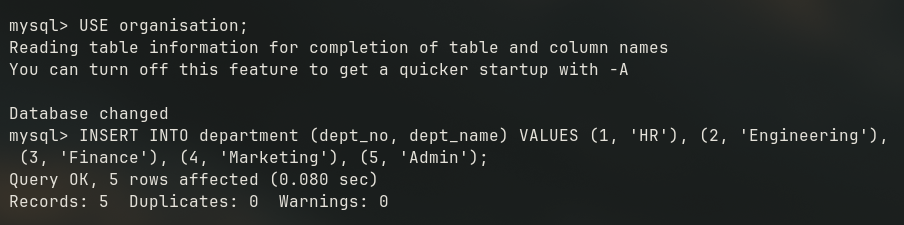
\includegraphics[width=0.88\linewidth,height=2.0cm,keepaspectratio]{Exp3-1.png}
    \caption{Populating tuples into the \texttt{department} table.}
    \label{fig:exp3_dept}
\end{figure}

\begin{figure}[H]
    \centering
    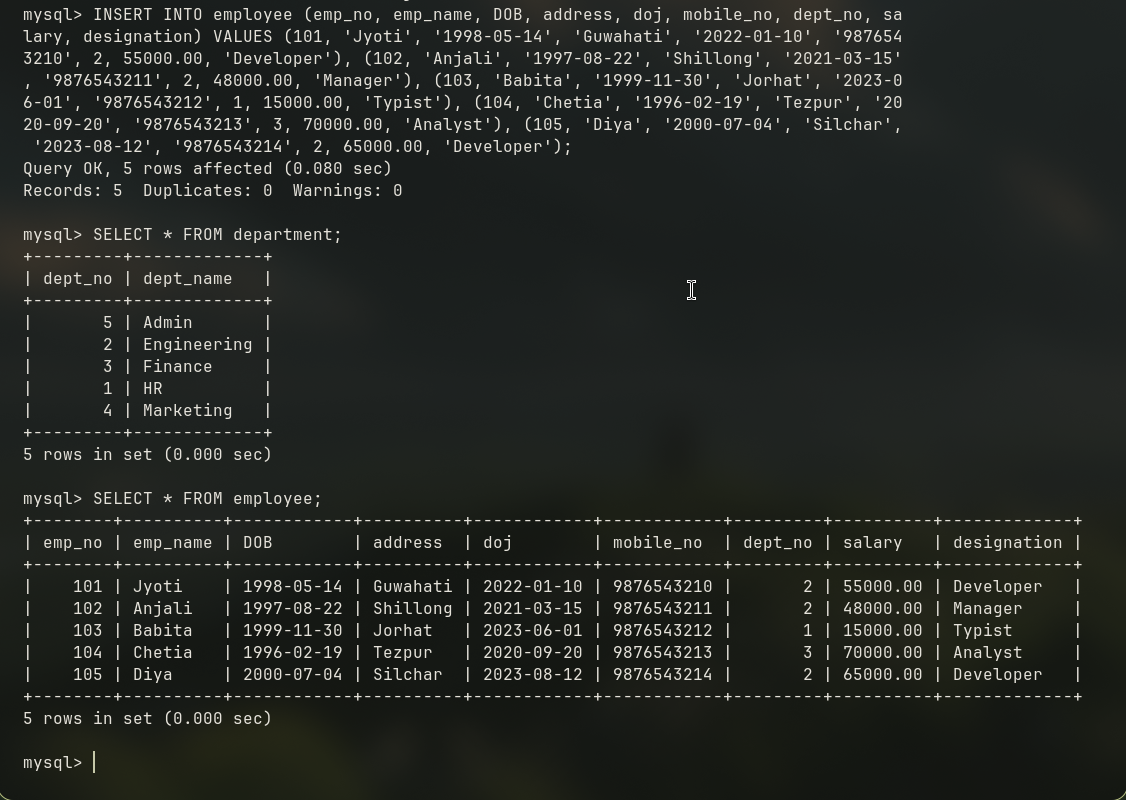
\includegraphics[width=0.88\linewidth,height=5.4cm,keepaspectratio]{Exp3-2.png}
    \caption{Populating tuples into the \texttt{employee} table and verifying records.}
    \label{fig:exp3_emp}
\end{figure}

\newpage

\subsubsection*{Part 2: Filtering, Sorting, Distinct, and Grouping Queries}
Queries filtering by department, sorting descending by salary, filtering ranges via \texttt{BETWEEN}, eliminating duplicate designations via \texttt{DISTINCT}, and grouping departmental expenditures:

\begin{lstlisting}[caption={Executing selective queries, sorting, distinct, and updates}]
-- Employees in Dept 2 and descending salary ordering
SELECT emp_no, emp_name FROM employee WHERE dept_no = 2;
SELECT emp_no, emp_name, designation, dept_no, salary FROM employee ORDER BY salary DESC;

-- Salary range filtering and distinct designations
SELECT emp_no, emp_name FROM employee WHERE salary BETWEEN 20000 AND 50000;
SELECT DISTINCT designation FROM employee;

-- Departmental expenditure and updating Typist salary
SELECT dept_no, SUM(salary) AS total_salary FROM employee GROUP BY dept_no;
UPDATE employee SET salary = 25000 WHERE designation = 'Typist';
\end{lstlisting}

\begin{figure}[H]
    \centering
    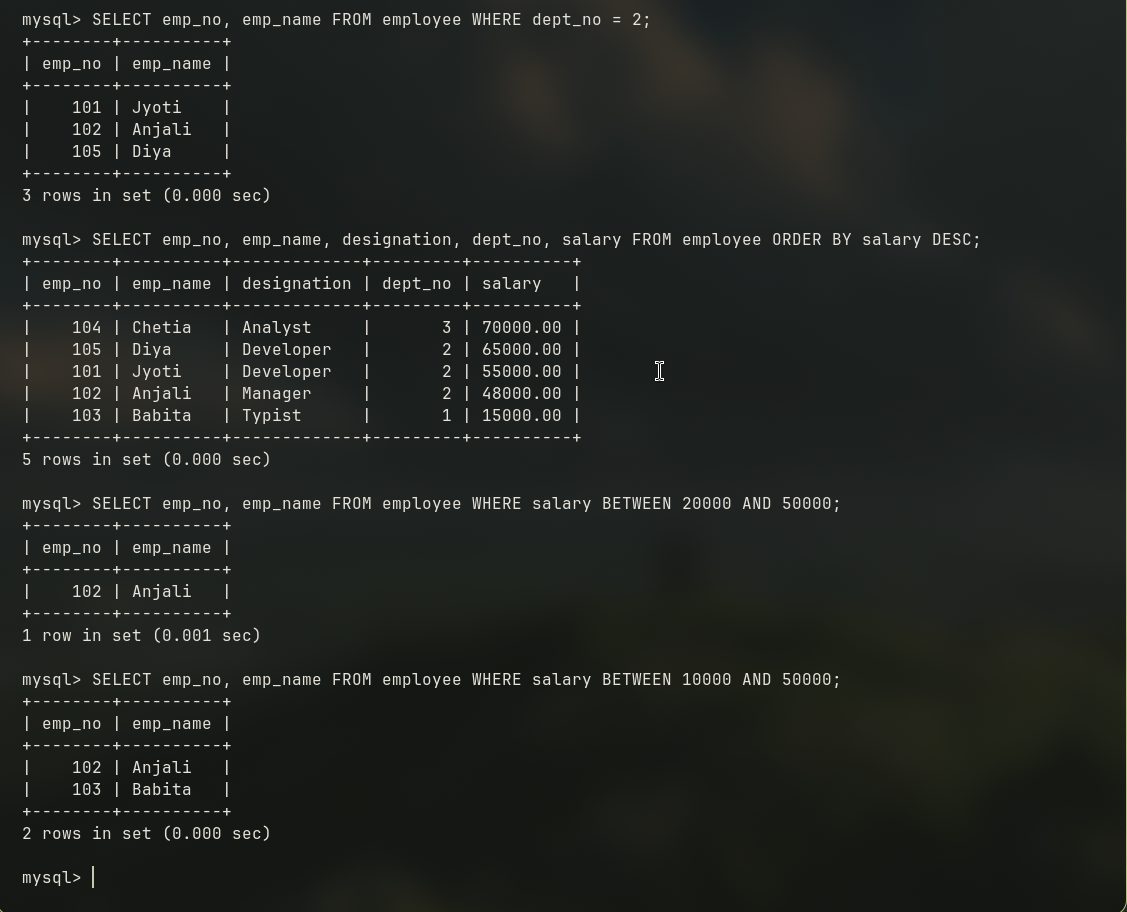
\includegraphics[width=0.88\linewidth,height=5.2cm,keepaspectratio]{Exp3-3.png}
    \caption{Filtering by department, descending sorting, and range condition queries.}
    \label{fig:exp3_filter}
\end{figure}

\begin{figure}[H]
    \centering
    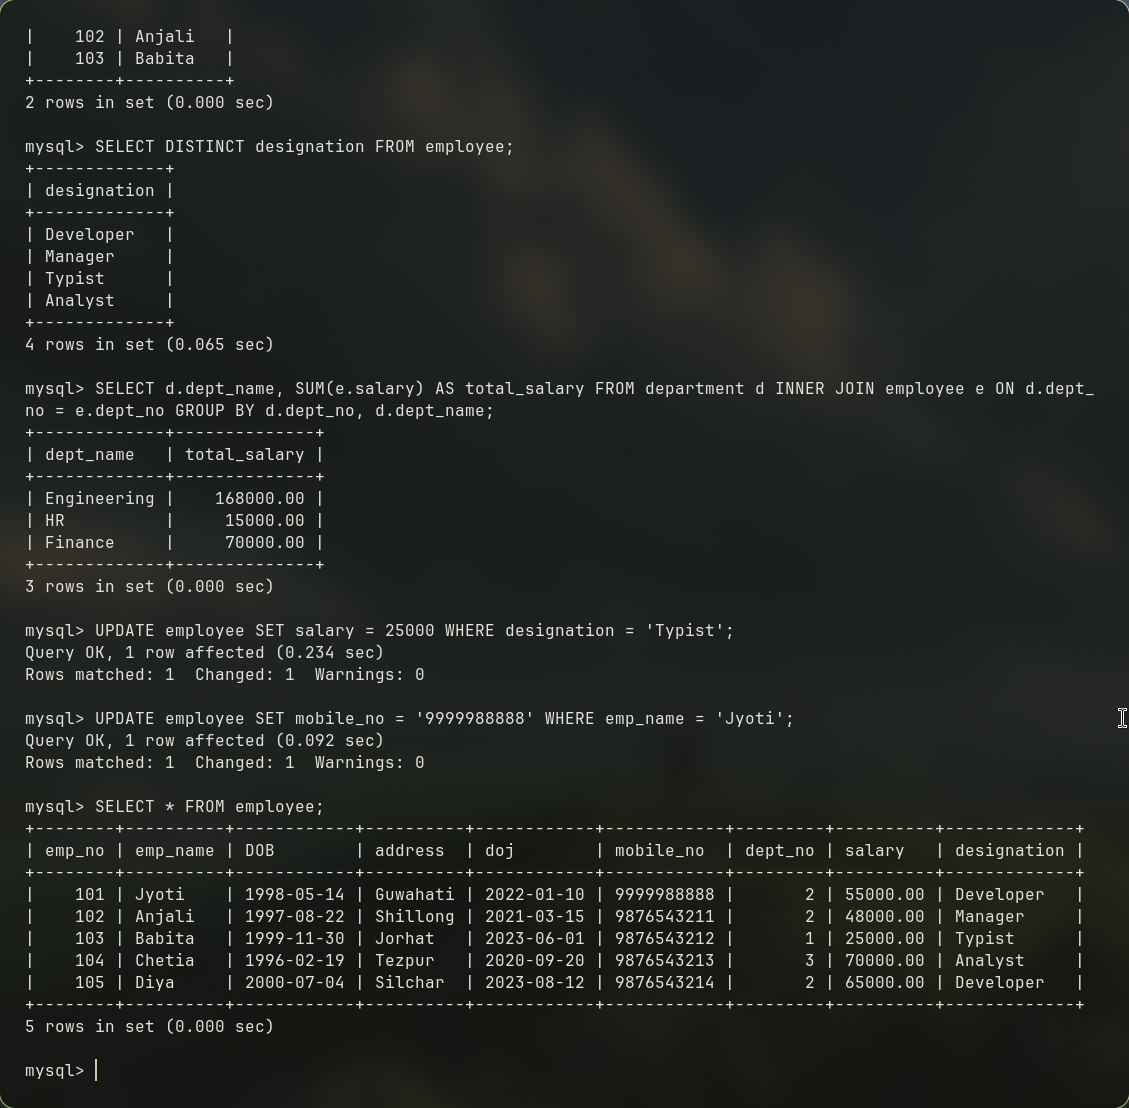
\includegraphics[width=0.88\linewidth,height=5.2cm,keepaspectratio]{Exp3-4.png}
    \caption{Distinct designations, grouped departmental summaries, and record modification.}
    \label{fig:exp3_group}
\end{figure}

\newpage

\subsubsection*{Part 3: Record Deletion and Filtered Group Aggregations}
Records matching a deletion predicate are removed using \texttt{DELETE}, and departments with aggregated salary expenditures exceeding 25,000 are queried using \texttt{HAVING}:

\begin{lstlisting}[caption={Executing DELETE and HAVING clause queries}]
-- Delete employees with salary equal to 70000
DELETE FROM employee WHERE salary = 70000;
SELECT * FROM employee;

-- Departments with total salary expenditure > 25000
SELECT dept_no, SUM(salary) AS total_salary 
FROM employee 
GROUP BY dept_no 
HAVING SUM(salary) > 25000;
\end{lstlisting}

\begin{figure}[H]
    \centering
    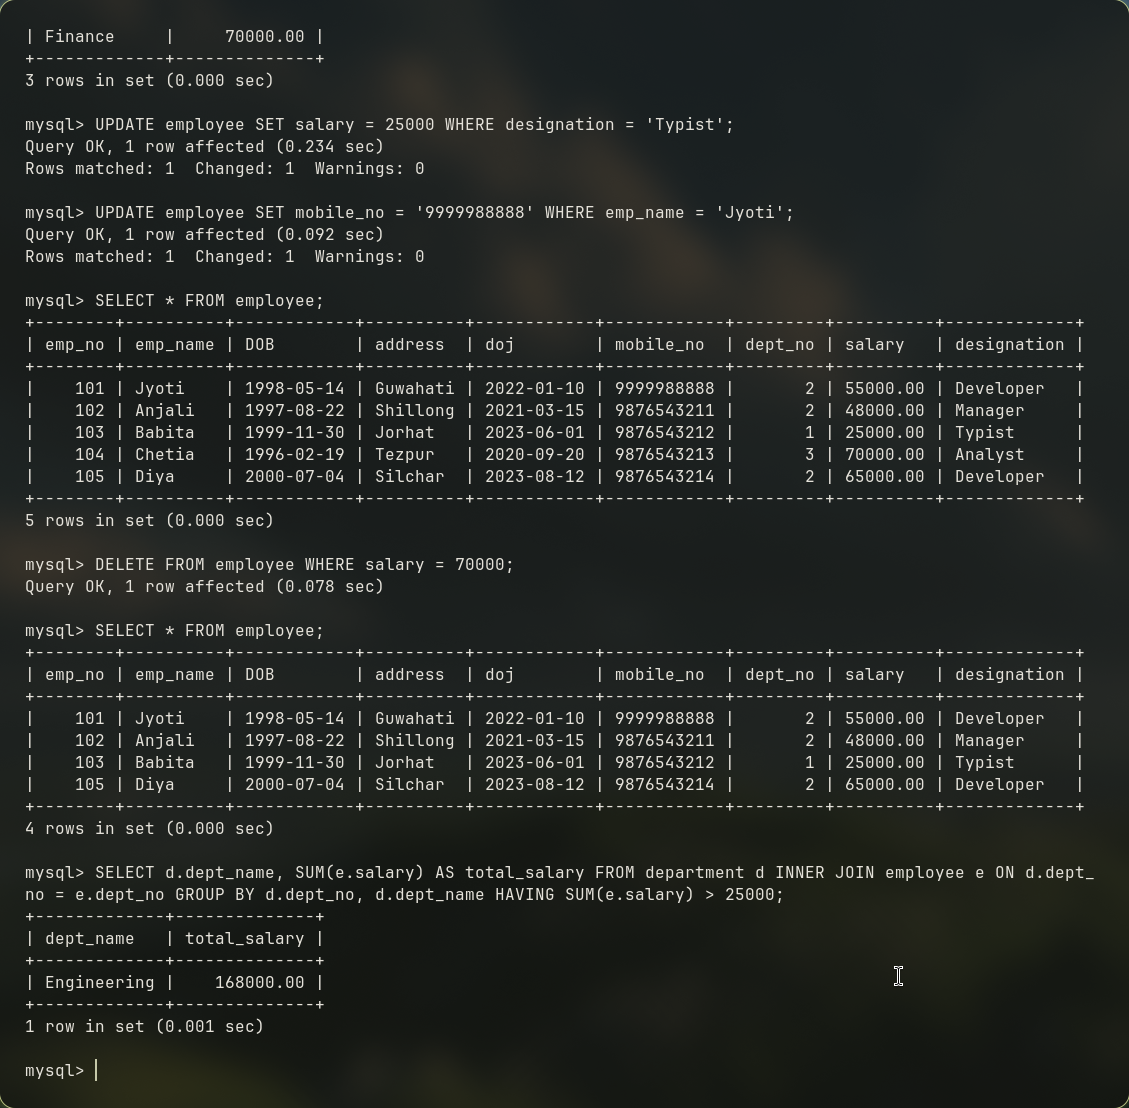
\includegraphics[width=0.88\linewidth,height=8.5cm,keepaspectratio]{Exp3-5.png}
    \caption{Tuple deletion verification and filtered group aggregations via \texttt{HAVING}.}
    \label{fig:exp3_delete_having}
\end{figure}

\subsection*{Result}
DML commands including record insertion, multi-criteria filtering, descending sorting, duplicate elimination, grouped aggregations, updates, and deletions were executed and verified successfully in MySQL.
